% !TEX TS-program = pdflatex
% !TEX encoding = UTF-8 Unicode

% This is a simple template for a LaTeX document using the "article" class.
% See "book", "report", "letter" for other types of document.

\documentclass[11pt]{article} % use larger type; default would be 10pt

\usepackage[utf8]{inputenc} % set input encoding (not needed with XeLaTeX)

%%% Examples of Article customizations
% These packages are optional, depending whether you want the features they provide.
% See the LaTeX Companion or other references for full information.

%%% PAGE DIMENSIONS
\usepackage{geometry} % to change the page dimensions
\geometry{top=3cm,bottom=3cm,left=3cm,right=3cm,letterpaper} % or letterpaper (US) or a5paper or....

\usepackage{graphicx} % support the \includegraphics command and options

% \usepackage[parfill]{parskip} % Activate to begin paragraphs with an empty line rather than an indent

%%% PACKAGES
\usepackage{booktabs} % for much better looking tables
\usepackage{array} % for better arrays (eg matrices) in maths
\usepackage{paralist} % very flexible & customisable lists (eg. enumerate/itemize, etc.)
\usepackage{epsfig}
\usepackage{verbatim} % adds environment for commenting out blocks of text & for better verbatim
\usepackage{subfig} % make it possible to include more than one captioned figure/table in a single float
\usepackage{amstext}
% These packages are all incorporated in the memoir class to one degree or another...

%%% HEADERS & FOOTERS
\usepackage{fancyhdr} % This should be set AFTER setting up the page geometry
\pagestyle{fancy} % options: empty , plain , fancy
\renewcommand{\headrulewidth}{0pt} % customise the layout...
\lhead{}\chead{}\rhead{}
\lfoot{}\cfoot{\thepage}\rfoot{}

%%% SECTION TITLE APPEARANCE
\usepackage{sectsty}
\allsectionsfont{\sffamily\mdseries\upshape} % (See the fntguide.pdf for font help)
% (This matches ConTeXt defaults)

%%% ToC (table of contents) APPEARANCE
\usepackage[nottoc,notlof,notlot]{tocbibind} % Put the bibliography in the ToC
\usepackage[titles,subfigure]{tocloft} % Alter the style of the Table of Contents
\renewcommand{\cftsecfont}{\rmfamily\mdseries\upshape}
\renewcommand{\cftsecpagefont}{\rmfamily\mdseries\upshape} % No bold!

%%% END Article customizations

%%% The "real" document content comes below...

\title{Minimizing Time Required For Graduation}
\author{Ruyi Cai \and Matthew Fonda \and Michael Hughes}
%\date{} % Activate to display a given date or no date (if empty),
         % otherwise the current date is printed 

\begin{document}
\maketitle

% Adds a table of contents. Comment out if we don't want this.
\tableofcontents
\pagebreak


\abstract{The Bachelor's Degree is designed to take four years to complete;
however, many students fail to complete it this amount of time. One of the
factors contributing to this is a lack of proper planning during the
registration phase. In this paper we present an algorithm to assist students in
constructing a schedule that works towards completing a degree in the shortest
amount of time possible.}


\section{Introduction} \subsection{Background} Registration can be a stressful
time for every student at the University of Washington. Without deliberate
planning, students must decide which classes to take on a quarterly basis. The
decision process involves considering factors such as quarterly class
offerings, the amount of credits, the prerequisites of the classes, time
conflicts, and how the choices in current quarter affect future quarters. The
University of Washington registration system provides a schedule finder;
however, it only takes into account time conflicts, and does not give advice on
how to pick the most ideal schedule. 

A student's graduation time may be extended because of his or her inability to
take a class that has limited offerings during that particular year.
Additionally, the advising office’s workload can also be increased due to the
changing plans and majors of students and their need for repeated advising. 

\subsection{Goal} Our goal is to alleviate the problematic situation by creating
a mathematical algorithm that accomplishes the following goal: given a student's
current state and preferred credit hours per quarter, produce a class schedule
that minimizes the number of quarters until graduation, eliminates time
conflicts, and eliminates prerequisite conflicts.

\subsection{Importance} The implementation of the algorithm as part of the
school’s registration system will benefit the students by enabling them to map
out their quarterly class schedules until graduation. Students will be able to
preview their ideal schedule, the length of time until graduation, and the
credit hours per quarter.  This will lead to better decision making for what
majors to pursue, and given the student's current state, which schedules are the
most ideal in terms of saving time and resources. This will also help students
save money, as they will be in school for fewer quarters. The university also
benefits from the reduced labor cost and increased efficiency of the advising
offices.

\section{Problem Description} We focus on the classes offered within the Math
department, although our algorithm and model can be easily extended to include
over departments. 

Every quarter the Math department offers a subset of classes from all of the
available courses, each class is offered during a certain subset of available
time periods. Since there are far more classes than time periods during the
regular five-day week there are inevitably time conflicts between courses that
a student could take. To graduate with a B.S. in Mathematics there are certain
classes that are required and then there are elective requirements too. Adding
to the problem is many classes cannot just be taken whenever they are available;
instead, certain prerequisites must be satisfied first. In the case of math
courses, there can be multiple different prerequisite sets that satisfy the
requirements for a class.

Our goal is to determine a schedule of classes from some starting point to
graduation that given the above properties minimizes the total number of
quarters needed. Explicitly: \\ Minimize the total
number of quarters needed to graduate subject to: \begin{enumerate} \item Only
taking courses during quarters they are available \item Only taking a course
once \item Never exceeding a preset number of credit hours per quarter \item
Never taking more than one class at a given time \item Always satisfying
a course's prerequisites prior to taking that course \end{enumerate}

\subsection{Definitions} We will now formalize some terms used in our paper.
\begin{itemize} \item A {\it course} refers to any course offered by the
University of Washington. A course has associated with it a name used in the
University of Washington time schedule, for example {\it MATH309}. A course also
has associated with it the quarters in which it is offered. Throughout this
paper, we will refer to these using their time schedule abbreviates: {\it F} for
Fall Quarter, {\it W} for Winter Quarter, {\it Sp} for Spring Quarter, and {\it
S} for Summer Quarter. Each course is also worth a specific amount of credits.
\item We refer to a specific instance of a course as a {\it course offering}.
Each course offering additionally has associated with it the time of the day at
which the course meets, the quarter it is being offered, and the section number
of the offering.  \end{itemize}

Additionally: \begin{itemize} \item Let $S$ be the set of courses required to be
taken in order to graduate. $S$ can be thought of as our goal state, and can
also contain elective courses a student simply wishes to take.  \item Let $T$ be
the set of courses a given student has already completed. If no courses have
been taken, this set may be empty.  \item Let $U$ be the set of all courses
a student could possibly ever take.  \item Let $P$ be a set of rules specifying
course prerequisites.  \item Let $l$ be the maximum number of credits a student
wishes to take during any given quarter.  \item Let $O$ be the set of all
50-minute time blocks between 8:30am and 7:30pm from Monday through Friday.
\end{itemize}

\subsection{Representing Prerequisites} Initially, we hoped to represent course
prerequisites using a directed acyclic graph. Each node was a course, and edges
existed between nodes $i$ and $j$ if and only if $i$ was a prerequisite for $j$.
However, it does not work in our model, and courses can have a complicated set
of multiple prerequisites.  For example, {\it MATH327} requires both $MATH126$
and $MATH300$, or just $MATH136$. 

\begin{figure} [ht] 
\begin{center} 
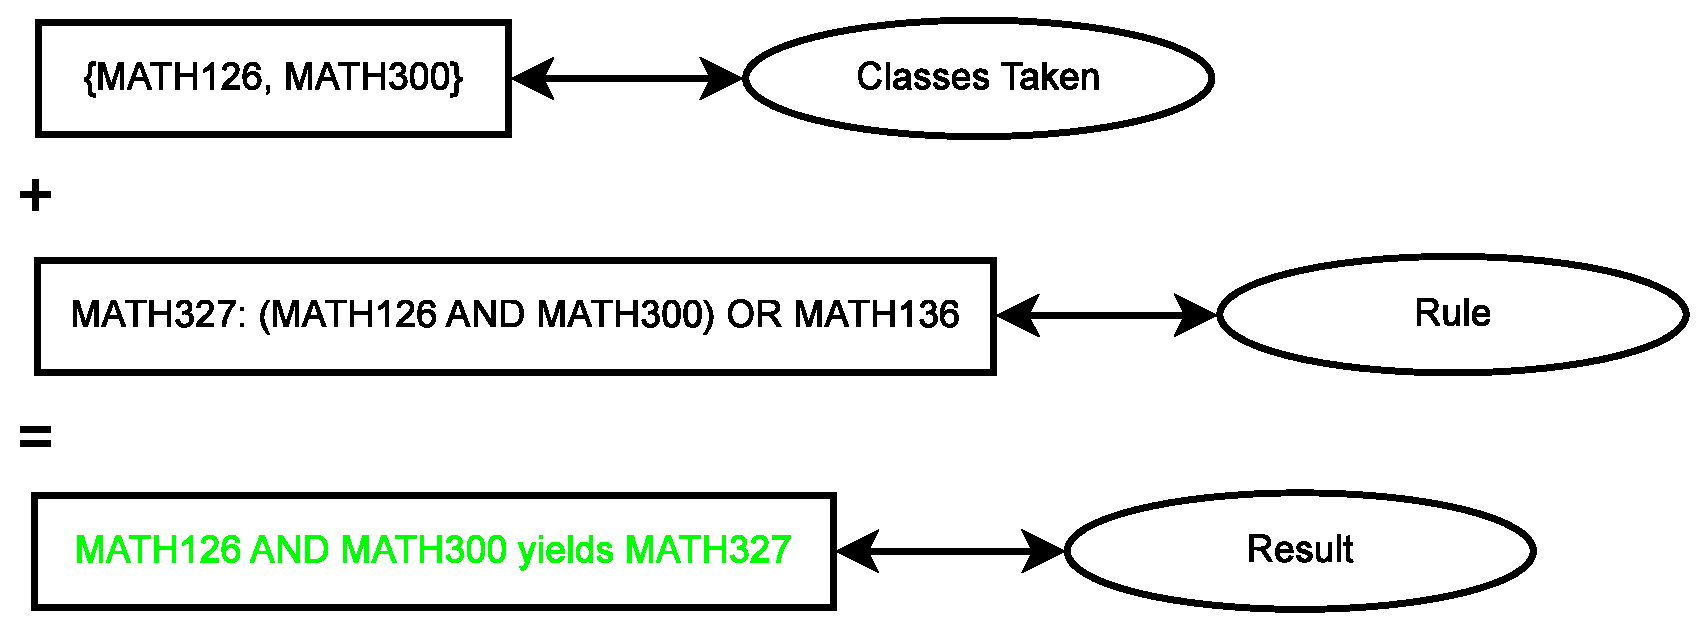
\includegraphics[scale=0.4]{prereq_logic_example} 
\end{center} 
\caption{Evaluation of a rule} 
\label{logic_ex} \end{figure}

To solve this issues, we introduce a set of rules for each course. Each rule is
a boolean expression represented in propositional logic in disjunctive normal
form. For example, the rule associated with $MATH327$ in fig~\ref{logic_ex} is
$$ \text{{\it MATH327: (MATH126 AND MATH300) OR MATH136}}.  $$ As previously
stated, we denote the set of all rules for all classes as $P$.

Furthermore, to determine if a given student is eligible to register for
a course offering, we can evaluate the rule for the course, where each clause
takes on the value true if a student has already taken the course, and false if
he or she hasn't. If the rule evaluates to true, then the student is eligible to
take the course; otherwise, the student is note. For example, consider
figure~\ref{logic_ex}, here a student has previously taken courses $MATH126$ and
$MATH300$. Since $MATH126$ and $MATH300$ have been taken, then those literals in
the rule for $MATH327$ evaluate to true and therefore the entire rule is true.
Since the entire rule is true, the student can take $MATH327$ when next
available.

\subsection{Initial Model and Tractability} With a static schedule it would be
possible to deterministically plan an entire schedule from start to finish,
unfortunately we have neither the computational resources nor the luxury of
a static schedule to do plan. From the student’s point of view, although there
are some classes that are offered every quarter, senior electives are not, and
sometimes it cannot be predicted more than one quarter in advance when a senior
elective will be offered. Even given perfect information, where we know the
possible class schedules for every quarter we face another problem; finding the
best possible schedule reduces to enumerating possible class schedules for every
quarter until the graduation requirements are satisfied. Given that we cannot
predict in advance the conflicts between classes, we cannot even determine the
branching factor of the enumeration tree nor its depth. Since we can only
determine one quarter in advance, this suggests approaching the problem by using
heuristics to pick the best possible classes each quarter.

Instead of trying to solve the complete problem we chose to use the rolling
horizon approach used by Xiangtong et al \cite{xiangton:informs} when scheduling
classes for airlines. Our problem already has a well defined horizon
demarcation, the quarters. For the rest of the paper we focus on developing
methods to optimally pick classes in each quarter separately.

\section{Rolling Horizons Approach} We adapt a rolling horizons approach which
uses a heuristic to pick the best possible schedule for any given quarter, given
the classes offered during the quarter and the courses the student has
previously taken. We use a greedy algorithm that functions on a per-quarter
basis to accomplish this. The greedy algorithm greatly improves the tractability
of course scheduling over an initially unknown number of quarters.

We break our algorithm down into two main phases: determining available course
offering and selecting specific course offerings.

\subsection{Determining Available Course Offerings} We need to select the
classes we can currently take and then build conflict graphs for classes based
on the times they are offered. In this section, we let $L$ be the initially
empty set of course offerings a given student is eligible to take in the given
quarter, $q$.

\subsubsection{Procedure} We present the procedure for populating the set $L$ as
follows: \begin{enumerate} \item For each rule in $P$ we iterate over each
proposition in the rule, $p$, and check if $p \in T$. If $p \in T$ then we say
$p$ evaluates to true; otherwise, $p$ evaluates to false. We recall that each
rule is associated with a given course. If the entire rule evaluates to true,
then we add the course associated with it to $L$. Once this is complete, $L$
will consist of every course that could be taken based solely on prerequisites
that we have fulfilled.  \item We now prune this set by removing all courses
that are not offered in the current quarter. $L$ will necessarily now only
contain classes that we can take given the current quarter and the classes we
have already taken.  \item We now construct a conflict graph, $G_{conflict}$,
where every course offering in $L$ is a node, and there is an edge between two
nodes $i$ and $j$ if and only if the time of course offering $i$ overlaps the
time of course offering $j$.  \end{enumerate}

\subsubsection{Analysis} The selection procedure involves a lot of set queries
and iteration, but in asymptotic running time the algorithm is relatively quick.
Let $n$ be the total number of classes ever available to take, or in other
words, $n = \|U\|$. In the worst case, $P$ has a complex rule for all $n$
courses, and checking each rule in $P$ is linear in the number of propositions.
However, we know {\it a priori} from analysis of our data set that the largest
rule has twelve propositions, so we can bound the rule check time by a constant,
$C$, and therefore step one can be done in $O(Cn)$ time.

Continuing to step two, the worst case is when $L$ = $Q$. Checking whether
a course is offered in a given quarter can be done in constant time, and we have
$n$ courses to check, therefore step two can also be done in $O(Cn)$ time.

Finally, the last step is once again bounded by a constant and $n$. Considering
courses between 8:30am and 7:30pm, we have nine fifty-minute time periods, and
five days of the week, and therefore we have 45 time slots to check in our
conflict graph, again yielding $O(Cn)$ runtime.

Since we are dealing with asymptotic running time we will drop the constant
terms and combining all results yields an overall runtime of $O(n)$.

\subsection{Selection of Quarterly Classes} \subsubsection{Selection Procedure}
At this point in time, we know which course offerings are available for the
given student to register for, and we must now pick the most optimal ones.  We
present two ways of approaching quarterly class choice. We will initially encode
the class selection as a binary integer programming problem in spirit of the
methods presented by Dinkel et al \cite{dinkel:scheduling}. and Pritsker et al
\cite{prisker:informs}. A second approach developed by Yamada et al
\cite{yamada:heuristic} and Pferschy et al \cite{pferschy:kcg} is presented for
dealing with very large class choices where binary LP would be difficult solve.

\subsubsection{Heuristic Value Function} In order to determine which classes
should be picked in a given schedule, we use a heuristic function which assigns
each course offering a value. The higher the value of this function for a given
course offering is, the more likely the given course offering will be placed in
the schedule. Recalling that our goal is to minimize the total number of
quarters taken (and implicitly, maximize the total number of courses taken per
quarter). Our heuristic function should give higher value to course offerings
that will help us achieve this goal. One component to the heuristic function
then must be the number of dependent courses a given course offering has. If
a course satisfies many prerequisites, then we know that there are many courses
that we cannot complete without it, so we want our heuristic function to favor
it. 

Additionally, we know that not every course is offered every quarter. If
a course is not offered until the following year, we could potentially add an
entire year to the schedule. This is a situation we hope to avoid. Our heuristic
function must therefore consider how often and how far in the future a given
course is offered. For example, if we are deciding between two course offering
that are identical except one is offered once a year, and the other is offered
three times a year, we want to take the course only offered once a year, as we
won't have the opportunity to take it for another entire year.

\begin{figure} [ht]
    \begin{center}
        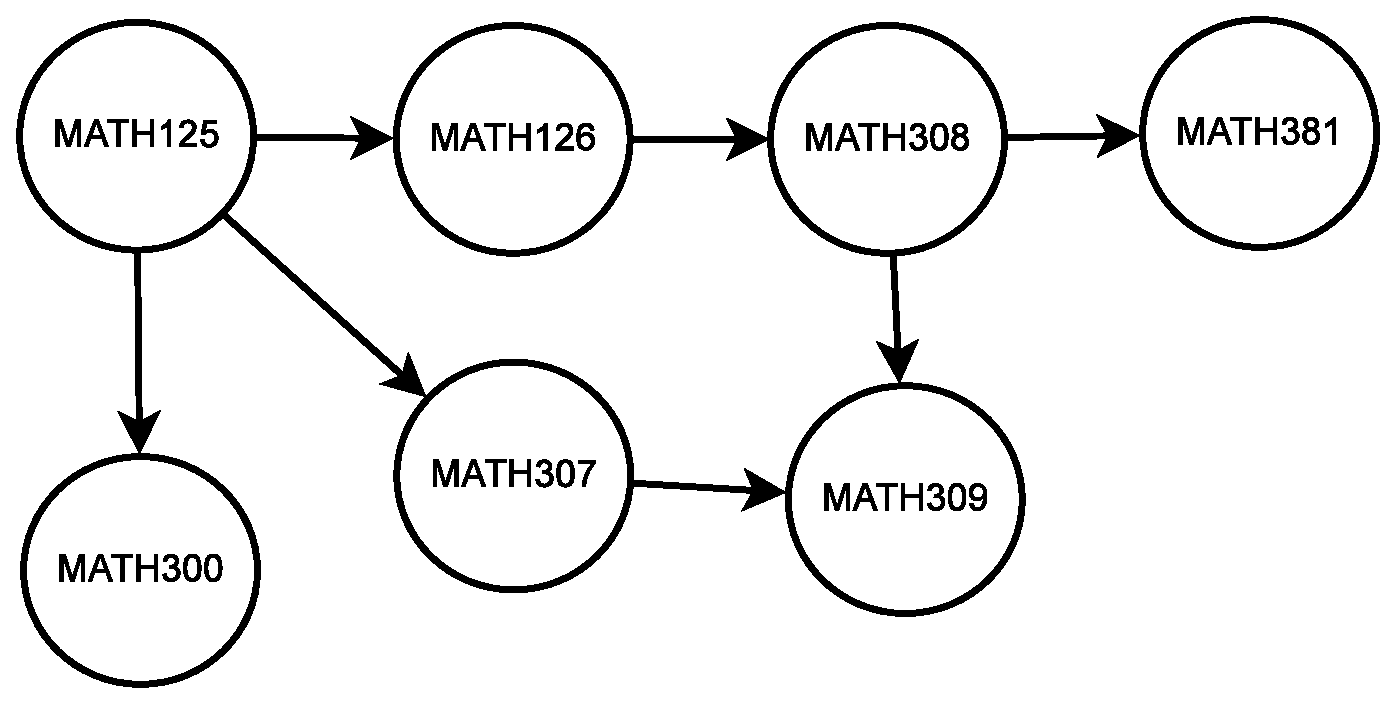
\includegraphics[scale=0.35]{more_prereq_tree}
    \end{center}
    \caption{A Prerequisite DAG}
    \label{prereq}
\end{figure}

We these considerations in mind, we begin to develop our heuristic function. In
order to define our heuristic function, we must first define some auxiliary
functions on course offering.  \begin{itemize} \item Let $TimeFromNow(c, q)$ be
difference in quarters between the current quarter, $q$, and the next quarter
a given course offering, $c$, is offered. As there are four quarters, the range
of this function is $\{0, 1, 2, 3\}$.  \item Let $Quarters(c)$ be the number of
quarters per year a given course, $c$, is offered. As there are four quarters,
the range of this function is $\{0, 1, 2, 3, 4\}$.  \item Let $Dependents(c)$ be
the number of course that either directly or indirectly require a given course,
$c$. In Figure~\ref{prereq}, $Dependents(MATH125)$ = 6 while
$Dependents(MATH307)$ = 1 \end{itemize}

With these functions defined, we can now define our heuristic function:

\begin{equation} 
    Value(c) = 1 + \alpha * Dependents(c) + \beta * TimeFromNow(c,q) 
    - \gamma * Quarters(c)
    \label{value_func}
\end{equation} 

Where $c$ is a given course offering,
$q$ is the current quarter, and $\alpha$, $\beta$, and $\gamma$ are real
numbers, giving a weight to piece of the heuristic. The scalars are determined
experimentally.

\subsubsection{Formulation as Binary Integer Program} We can now formulate
a binary linear programming problem. Before stating the linear
program, we must first define some variables used in it: 

\begin{itemize}
    \item $ X_i = \left\{ \begin{array}{lr} 1 \text{ if we take } X_i\\ 0 \text{ if
we don't take } X_i \end{array} \right. $ 
    \item For all $t \in O$, we let $t$ represent the conflict graph of classes
    at time period $t$.
    \item Let $m = \|L\|$.  
\end{itemize} 
We now state our problem as follows: 
Maximize: 

\begin{equation}
    \text{Value of Quarter} = \sum_{i=1}^m Value(c_i) * X_i
    \label{qtr_val}
\end{equation}
Subject To:
\begin{equation}
    \sum_{i=1}^m Weight(c_i) * X_i \leq l, 
    \label{weight_lim}
\end{equation}

\begin{equation}
    \forall t \in O,X_i+X_j \leq 1, \forall \text{ pairs } (X_i,X_j) \in t
    \label{time_con}
\end{equation}

\begin{equation}
   X_i + X_j \leq 1, \forall \text{ pairs } (X_i,X_j) \text{ where } X_i \text{and} X_j \text{ are offerings of
   the same course}
    \label{course_con}
\end{equation}

The linear program
can be interpreted as follows: \begin{itemize} \item The value of a quarter is
the total number of courses taken that quarter.  \item In each quarter, the
total number of credits cannot exceed the specified limit.  \item Only one
course can be taken in one particular time slot \item A course can only be taken
or not taken. In other words, decision variables are binary.  \item Each
non-zero decision variable in the optimal solution represents a class we will
take.  \end{itemize}

Each of the equations based on eqn.~\ref{time_con} ensure that we only take one class per 
time period per day. Also this linear program is ‘nice’ in that it always has 
feasible origin (don’t take any classes), and that the simplest formulation 
is already in standard form.

As noted in the reference literature this is actually a (strongly) NP-complete
problem as described \cite{pferschy:kcg}. For the rest of this section we
consider an alternative formulation of class selection as a knapsack problem
with conflict graphs and suggest the use a technique developed by Yamada et. al.
\cite{yamada:heuristic}.

We begin by simplifying $G_{conflict}$ to be a fully connected graph by adding
dummy nodes $v'$ and insert edges that connect $v'$ to every other node in the
graph. To ensure that $v'$ does not alter the final optimal solution, we assign
it the following properties: \begin{itemize} \item $Weight(v') = l+1$ \item
$Value(v') = 0$ \end{itemize} As the weight of our dummy node is greater than
our credit limit, and it's value is zero, we know that it will never appear in
the optimal solution. With the above reasoning we show for our case of class
schedule that Pferschy and Schauer's \cite{pferschy:kcg} claim that adding
a dummy node without loss of generality holds. We can now conveniently write the
class picking problem as the knapsack with conflict graphs problem (KCG): 

Maximize:

\begin{equation}
    \text{Value of Quarter} = \sum_{i=1}^m Value(c_i) * X_i
\end{equation}

Subject To: 

\begin{equation}
\sum_{i=1}^m Weight(c_i) * X_i \leq l,
\end{equation}

\begin{equation}
X_i + X_j \leq 1 \text{ for all connected vertices } i, j \in G_{conflict},
\end{equation}

\begin{equation}
X_i \in \{0, 1\}
\end{equation}

For versions of this problem in the low hundreds of variables it is possible 
to solve this problem exactly using modern LP solving software 
\cite{yamada:heuristic}. In our case, just solving for the optimal classes for 
a single major fits well into the scope of a few hundred (or even just tens of) 
variables. For multiple majors or to consider class selection
for distribution and elective requirements, however the number of classes
balloons significantly and the KCG problem becomes much harder. For this version
of the problem we suggest using the techniques used by Yamada et al
\cite{yamada:heuristic}, which we briefly outline below.

\subsubsection{Relaxation and Implicit Enumeration} \begin{enumerate} \item
Develop upper bound on value by solving a continuous version knapsack problem
generated by a Lagrangian relaxation of our problem. Let $X_i$ be a continuous
variable with $0 \leq X_i \leq 1$, and shift the time constraints into the
objective function by using a penalty of $\lambda$ when the constraint is
violated.  \item Use the upper bound developed above with the pruning rules
suggested by Yamada et al \cite{yamada:heuristic} to do implicit enumeration of
the possible choices.  \end{enumerate}

In Yamada et al’s \cite{yamada:heuristic} numerical runtime analysis they found
this algorithm ran very favorably against solving the same problem using popular
linear programming solvers. There is one problem that we should briefly address,
because the number of periods of available classes per week is relatively small
the conflict rate for a large number of class is relatively higher than Yamada
et al’s 2\% maximal conflict rate for their experiments. Our data has
a significant mitigating factor though, knapsack problems in general are
exponential in terms of the number of choices and the total weight capacity.
Realistically the total weight capacity is going to be 20 credits or less which
is between 1\% and 2\% of the figures used by Yamada \cite{yamada:heuristic} and
also our total number of choices is in many cases (particular just the classes
in a particular major) less than 200. Giving the size and type of data in our
set the higher conflict rate is less of a concern and Yamada et al’s algorithm
should still be efficient.

\section{Computational Results} In this section we will outline results obtained
by running computer simulations of schedule picking. We will computationally
examine what parameters in our heuristic function produce the most desirable
schedules.

\bibliography{paper_references}{} \bibliographystyle{plain} \end{document}
